\documentclass[14pt]{extbook}
\usepackage{multicol, enumerate, enumitem, hyperref, color, soul, setspace, parskip, fancyhdr} %General Packages
\usepackage{amssymb, amsthm, amsmath, latexsym, units, mathtools} %Math Packages
\everymath{\displaystyle} %All math in Display Style
% Packages with additional options
\usepackage[headsep=0.5cm,headheight=12pt, left=1 in,right= 1 in,top= 1 in,bottom= 1 in]{geometry}
\usepackage[usenames,dvipsnames]{xcolor}
\usepackage{dashrule}  % Package to use the command below to create lines between items
\newcommand{\litem}[1]{\item#1\hspace*{-1cm}\rule{\textwidth}{0.4pt}}
\pagestyle{fancy}
\lhead{Progress Quiz 6}
\chead{}
\rhead{Version C}
\lfoot{4563-7456}
\cfoot{}
\rfoot{Summer C 2021}
\begin{document}

\begin{enumerate}
\litem{
First, find the equation of the line containing the two points below. Then, write the equation in the form $ y=mx+b $ and choose the intervals that contain $m$ and $b$.\[ (-4, -5) \text{ and } (-8, 4) \]\begin{enumerate}[label=\Alph*.]
\item \( m \in [-5.25, 0.75] \hspace*{3mm} b \in [12.7, 14.1] \)
\item \( m \in [2.25, 6.25] \hspace*{3mm} b \in [19.8, 22.7] \)
\item \( m \in [-5.25, 0.75] \hspace*{3mm} b \in [-2.2, 2] \)
\item \( m \in [-5.25, 0.75] \hspace*{3mm} b \in [-17.3, -13.9] \)
\item \( m \in [-5.25, 0.75] \hspace*{3mm} b \in [11.7, 12.2] \)

\end{enumerate} }
\litem{
Solve the linear equation below. Then, choose the interval that contains the solution.\[ \frac{5x -3}{3} - \frac{9x + 5}{2} = \frac{-3x + 9}{5} \]\begin{enumerate}[label=\Alph*.]
\item \( x \in [-0.3, 0.3] \)
\item \( x \in [-4.5, -0.7] \)
\item \( x \in [-6.6, -4.2] \)
\item \( x \in [-9.5, -7] \)
\item \( \text{There are no real solutions.} \)

\end{enumerate} }
\litem{
Write the equation of the line in the graph below in Standard Form $Ax+By=C$. Then, choose the intervals that contain $A, B, \text{ and } C$.
\begin{center}
    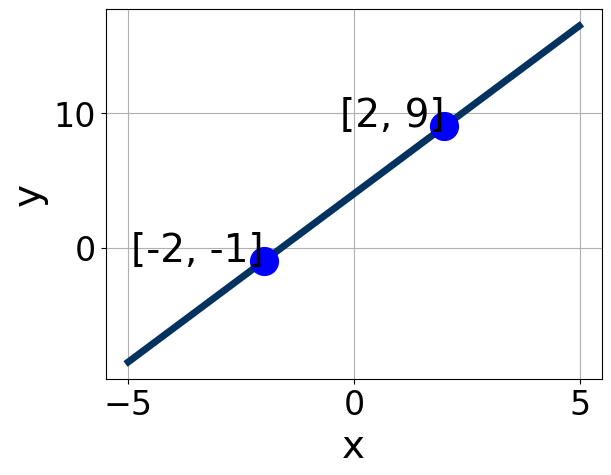
\includegraphics[width=0.5\textwidth]{../Figures/linearGraphToStandardC.png}
\end{center}
\begin{enumerate}[label=\Alph*.]
\item \( A \in [-2.5, 3.5], \hspace{3mm} B \in [-0.1, 1.48], \text{ and } \hspace{3mm} C \in [3, 7] \)
\item \( A \in [-2.5, 3.5], \hspace{3mm} B \in [-1.5, -0.51], \text{ and } \hspace{3mm} C \in [-5, -3] \)
\item \( A \in [4, 6], \hspace{3mm} B \in [1.69, 3.53], \text{ and } \hspace{3mm} C \in [8, 15] \)
\item \( A \in [4, 6], \hspace{3mm} B \in [-2.2, -1.73], \text{ and } \hspace{3mm} C \in [-10, -7] \)
\item \( A \in [-9, -3], \hspace{3mm} B \in [1.69, 3.53], \text{ and } \hspace{3mm} C \in [8, 15] \)

\end{enumerate} }
\litem{
Solve the equation below. Then, choose the interval that contains the solution.\[ -13(5x + 19) = -3(-11x + 15) \]\begin{enumerate}[label=\Alph*.]
\item \( x \in [1.3, 3.6] \)
\item \( x \in [-9.8, -7.4] \)
\item \( x \in [-2.7, -1.6] \)
\item \( x \in [-3.3, -2.5] \)
\item \( \text{There are no real solutions.} \)

\end{enumerate} }
\litem{
Find the equation of the line described below. Write the linear equation in the form $ y=mx+b $ and choose the intervals that contain $m$ and $b$.\[ \text{Parallel to } 5 x - 7 y = 14 \text{ and passing through the point } (10, 3). \]\begin{enumerate}[label=\Alph*.]
\item \( m \in [-1.26, -0.2] \hspace*{3mm} b \in [8.8, 10.4] \)
\item \( m \in [0.07, 1.38] \hspace*{3mm} b \in [-8.4, -4.5] \)
\item \( m \in [0.07, 1.38] \hspace*{3mm} b \in [3.2, 6.7] \)
\item \( m \in [1.02, 1.91] \hspace*{3mm} b \in [-4.3, -1.4] \)
\item \( m \in [0.07, 1.38] \hspace*{3mm} b \in [-4.3, -1.4] \)

\end{enumerate} }
\litem{
Write the equation of the line in the graph below in Standard Form $Ax+By=C$. Then, choose the intervals that contain $A, B, \text{ and } C$.
\begin{center}
    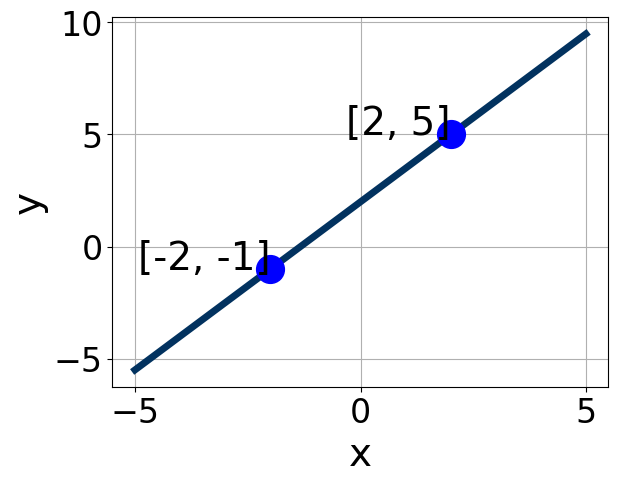
\includegraphics[width=0.5\textwidth]{../Figures/linearGraphToStandardCopyC.png}
\end{center}
\begin{enumerate}[label=\Alph*.]
\item \( A \in [-4.5, -2.5], \hspace{3mm} B \in [1.58, 2.76], \text{ and } \hspace{3mm} C \in [3.79, 5.34] \)
\item \( A \in [-2.8, 0.7], \hspace{3mm} B \in [0.02, 1.16], \text{ and } \hspace{3mm} C \in [0.61, 2.29] \)
\item \( A \in [1, 5.7], \hspace{3mm} B \in [-3.02, -1.46], \text{ and } \hspace{3mm} C \in [-6.48, -3.39] \)
\item \( A \in [-2.8, 0.7], \hspace{3mm} B \in [-1.76, -0.98], \text{ and } \hspace{3mm} C \in [-3.88, -1.87] \)
\item \( A \in [1, 5.7], \hspace{3mm} B \in [1.58, 2.76], \text{ and } \hspace{3mm} C \in [3.79, 5.34] \)

\end{enumerate} }
\litem{
Find the equation of the line described below. Write the linear equation in the form $ y=mx+b $ and choose the intervals that contain $m$ and $b$.\[ \text{Parallel to } 5 x - 7 y = 10 \text{ and passing through the point } (3, 2). \]\begin{enumerate}[label=\Alph*.]
\item \( m \in [1.06, 2.08] \hspace*{3mm} b \in [-0.6, 0.04] \)
\item \( m \in [0.14, 0.72] \hspace*{3mm} b \in [-0.6, 0.04] \)
\item \( m \in [-0.75, -0.33] \hspace*{3mm} b \in [4.03, 4.42] \)
\item \( m \in [0.14, 0.72] \hspace*{3mm} b \in [-1, -0.92] \)
\item \( m \in [0.14, 0.72] \hspace*{3mm} b \in [-0.13, 0.34] \)

\end{enumerate} }
\litem{
Solve the equation below. Then, choose the interval that contains the solution.\[ -6(18x -14) = -10(5x + 7) \]\begin{enumerate}[label=\Alph*.]
\item \( x \in [2.61, 2.82] \)
\item \( x \in [0.18, 0.34] \)
\item \( x \in [-0.04, 0.22] \)
\item \( x \in [-0.6, -0.1] \)
\item \( \text{There are no real solutions.} \)

\end{enumerate} }
\litem{
First, find the equation of the line containing the two points below. Then, write the equation in the form $ y=mx+b $ and choose the intervals that contain $m$ and $b$.\[ (10, 4) \text{ and } (9, -7) \]\begin{enumerate}[label=\Alph*.]
\item \( m \in [9, 13] \hspace*{3mm} b \in [106, 110] \)
\item \( m \in [9, 13] \hspace*{3mm} b \in [-107, -103] \)
\item \( m \in [9, 13] \hspace*{3mm} b \in [-6, -2] \)
\item \( m \in [-15, -8] \hspace*{3mm} b \in [92, 93] \)
\item \( m \in [9, 13] \hspace*{3mm} b \in [-23, -13] \)

\end{enumerate} }
\litem{
Solve the linear equation below. Then, choose the interval that contains the solution.\[ \frac{-4x + 9}{3} - \frac{-3x -4}{8} = \frac{-5x + 6}{4} \]\begin{enumerate}[label=\Alph*.]
\item \( x \in [-0.5, 3.5] \)
\item \( x \in [-8.86, -5.86] \)
\item \( x \in [-4.43, -1.43] \)
\item \( x \in [-25, -22] \)
\item \( \text{There are no real solutions.} \)

\end{enumerate} }
\end{enumerate}

\end{document}